\section{Results}
\label{sec:results}
In this section we describe the results obtained from our simulations.  The 
section is divided into two parts. In the first part we present some general 
results of our simulations, reviewing the general behaviour of our 
simulations. In the second part we present the results of our attempts to 
replicate the phenomena outlined in section~\ref{sec:article-results}. A 
discussion of these results is presented in section~\ref{sec:discussion}.

\subsection{The basics}
In this section we describe some general results of our simulations. 
First we present the scenarios that we have simulated, and the parameters 
used in the simulations. We then move on to comment on the general behaviour 
of the pedestrians in our simulations and within which limits the simulations 
give reasonable results.

\subsubsection{Scenarios}
As outlined in section~\ref{sec:scenario-presentation}, we will simulate two 
different main scenarios, a square room and a corridor, with some variations 
of the latter. Counting the variations, we simulate three different scenarios: 
A rectangle shaped room with a door in the middle of one of the walls, and a 
normal corridor and a corridor with a bottleneck in the middle.  In the 
corridors we do simulations of both uni-- and birectional flow. Images of each 
of these scenarios are presented in figure \ref{fig:simulated-cases}.

\begin{figure}[h]
    \centering
    \subfloat[Square room.]{
        \resizebox{0.45\textwidth}{!}{\begin{tikzpicture}

\end{tikzpicture}
}
        \label{subfig:image-square-room}
    }\\
    \subfloat[Corridor.]{
        \resizebox{0.45\textwidth}{!}{\begin{tikzpicture}
\draw[color=blue] (11.86,0.21) circle (0.21);
\draw[color=blue] (12.23,-1.26) circle (0.19);
\draw[color=blue] (11.20,0.43) circle (0.21);
\draw[color=blue] (11.84,1.02) circle (0.20);
\draw[color=blue] (12.21,-0.58) circle (0.20);
\draw[color=blue] (10.65,0.54) circle (0.19);
\draw[color=blue] (11.47,-0.42) circle (0.20);
\draw[color=blue] (10.31,-0.21) circle (0.20);
\draw[color=blue] (10.09,0.52) circle (0.20);
\draw[color=blue] (9.67,-0.59) circle (0.21);
\draw[color=blue] (10.79,-0.65) circle (0.19);
\draw[color=blue] (8.99,-0.61) circle (0.17);
\draw[color=blue] (8.40,0.19) circle (0.20);
\draw[color=blue] (8.02,-0.08) circle (0.19);
\draw[color=blue] (9.02,-0.04) circle (0.18);
\draw[color=blue] (9.53,0.55) circle (0.19);
\draw[color=blue] (9.70,-0.02) circle (0.21);
\draw[color=blue] (8.54,-0.52) circle (0.20);
\draw[color=blue] (7.38,-0.12) circle (0.20);
\draw[color=blue] (7.99,-0.62) circle (0.20);
\draw[color=blue] (9.05,0.58) circle (0.19);
\draw[color=blue] (7.12,-0.63) circle (0.21);
\draw[color=blue] (6.73,-0.23) circle (0.20);
\draw[color=blue] (6.29,-0.68) circle (0.21);
\draw[color=blue] (6.99,0.51) circle (0.20);
\draw[color=blue] (5.63,-0.56) circle (0.20);
\draw[color=blue] (6.39,0.67) circle (0.21);
\draw[color=blue] (5.90,0.69) circle (0.20);
\draw[color=blue] (5.26,-0.79) circle (0.19);
\draw[color=blue] (6.07,-0.20) circle (0.21);
\draw[color=blue] (5.24,0.63) circle (0.20);
\draw[color=blue] (6.51,0.18) circle (0.19);
\draw[color=blue] (5.72,0.30) circle (0.21);
\draw[color=blue] (8.44,0.68) circle (0.19);
\draw[color=blue] (2.95,-0.67) circle (0.19);
\draw[color=blue] (4.81,-0.04) circle (0.23);
\draw[color=blue] (4.80,0.54) circle (0.19);
\draw[color=blue] (4.50,-0.67) circle (0.20);
\draw[color=blue] (7.76,0.48) circle (0.19);
\draw[color=blue] (3.48,0.17) circle (0.19);
\draw[color=blue] (5.48,-0.06) circle (0.21);
\draw[color=blue] (2.24,-0.57) circle (0.19);
\draw[color=blue] (1.65,-0.50) circle (0.21);
\draw[color=blue] (4.42,0.69) circle (0.19);
\draw[color=blue] (3.85,0.57) circle (0.20);
\draw[color=blue] (3.64,-0.48) circle (0.20);
\draw[color=blue] (4.38,0.16) circle (0.19);
\draw[color=blue] (3.29,0.72) circle (0.21);
\draw[color=blue] (5.10,-0.43) circle (0.20);
\draw[color=blue] (2.35,0.58) circle (0.20);
\draw[color=blue] (4.16,-0.31) circle (0.20);
\draw[color=blue] (1.83,0.41) circle (0.22);
\draw[color=blue] (0.60,0.09) circle (0.20);
\draw[color=blue] (0.58,0.63) circle (0.20);
\draw[color=blue] (2.99,0.36) circle (0.19);
\draw[color=blue] (1.14,0.55) circle (0.19);
\draw[color=blue] (2.57,-0.05) circle (0.20);
\draw[color=blue] (3.26,-0.22) circle (0.20);
\draw[color=blue] (1.18,-0.57) circle (0.20);
\draw[color=blue] (1.51,0.01) circle (0.20);
\draw[color=blue] (0.65,-0.60) circle (0.21);
\draw[color=blue] (0.26,-0.23) circle (0.19);
\draw[color=blue] (-0.31,0.02) circle (0.21);
\draw[color=blue] (-0.07,-0.61) circle (0.21);
\draw[color=blue] (-1.00,0.09) circle (0.21);
\draw[color=blue] (-1.75,-0.08) circle (0.22);
\draw[color=blue] (0.12,0.55) circle (0.20);
\draw[color=blue] (-0.42,0.60) circle (0.20);
\draw[color=blue] (-0.61,-0.66) circle (0.20);
\draw[color=blue] (-0.94,-0.42) circle (0.20);
\draw[color=blue] (-1.60,0.52) circle (0.21);
\draw[color=blue] (-1.55,-0.61) circle (0.19);
\draw[color=blue] (-0.98,0.62) circle (0.20);
\draw[color=blue] (-2.45,-0.06) circle (0.22);
\draw[color=blue] (-2.47,-0.62) circle (0.20);
\draw[color=blue] (-2.98,-0.47) circle (0.20);
\draw[color=blue] (-2.28,0.60) circle (0.20);
\draw[color=blue] (-2.73,0.44) circle (0.20);
\draw[color=blue] (-3.28,0.62) circle (0.19);
\draw[color=blue] (-3.42,-0.63) circle (0.20);
\draw[color=blue] (-3.33,0.00) circle (0.21);
\draw[color=blue] (-3.78,0.22) circle (0.20);
\draw[color=blue] (-4.13,0.63) circle (0.19);
\draw[color=blue] (-3.93,-0.47) circle (0.20);
\draw[color=blue] (-4.51,-0.59) circle (0.20);
\draw[color=blue] (-4.37,0.04) circle (0.19);
\draw[color=blue] (-4.83,0.05) circle (0.21);
\draw[color=blue] (-4.82,0.62) circle (0.20);
\draw[color=blue] (-5.52,0.56) circle (0.20);
\draw[color=blue] (-6.21,0.15) circle (0.21);
\draw[color=blue] (-5.77,-0.52) circle (0.20);
\draw[color=blue] (-5.02,-0.58) circle (0.19);
\draw[color=blue] (-5.36,-0.03) circle (0.20);
\draw[color=blue] (-6.42,-0.52) circle (0.19);
\draw[color=blue] (-7.00,-0.42) circle (0.20);
\draw[color=blue] (-6.46,0.67) circle (0.20);
\draw[color=blue] (-6.70,0.17) circle (0.21);
\draw[color=blue] (-7.57,-0.63) circle (0.20);
\draw[color=blue] (-7.49,-0.04) circle (0.22);
\draw[color=blue] (-7.99,0.07) circle (0.19);
\draw[color=blue] (-8.08,-0.58) circle (0.21);
\draw[color=blue] (-7.43,0.56) circle (0.19);
\draw[color=blue] (-8.40,0.54) circle (0.20);
\draw[color=blue] (-7.90,0.71) circle (0.21);
\draw[color=blue] (-8.61,-0.83) circle (0.21);
\draw[color=blue] (-8.52,-0.15) circle (0.20);
\draw[color=blue] (-8.75,0.38) circle (0.22);
\draw[color=blue] (-8.81,-0.37) circle (0.21);
\draw[color=blue] (-9.17,-0.13) circle (0.21);
\draw[color=blue] (-9.71,-0.45) circle (0.20);
%\node at (-12.50, 5.83) {t = 52.31};
\useasboundingbox (-12.50, -5.83) rectangle (12.50, 5.83);
\draw[color=black] (-10.00,1.00) -- (10.00,1.00);
\draw[color=black] (-10.00,-1.00) -- (10.00,-1.00);
\end{tikzpicture}
}
        \label{subfig:image-corridor}       
    }
    \subfloat[Bottleneck.]{
        \resizebox{0.45\textwidth}{!}{\begin{tikzpicture}
\draw[color=blue] (10.20,-0.82) circle (0.21);
\draw[color=blue] (11.02,-1.97) circle (0.20);
\draw[color=blue] (9.63,-0.94) circle (0.20);
\draw[color=blue] (11.62,-0.29) circle (0.19);
\draw[color=blue] (11.47,2.10) circle (0.18);
\draw[color=blue] (10.48,-2.41) circle (0.19);
\draw[color=blue] (5.77,0.15) circle (0.20);
\draw[color=blue] (9.33,1.17) circle (0.20);
\draw[color=blue] (11.70,0.48) circle (0.20);
\draw[color=blue] (10.58,-0.16) circle (0.20);
\draw[color=blue] (10.44,1.08) circle (0.19);
\draw[color=blue] (12.15,1.00) circle (0.18);
\draw[color=blue] (11.04,1.59) circle (0.19);
\draw[color=blue] (9.23,-0.44) circle (0.19);
\draw[color=blue] (6.84,-1.70) circle (0.20);
\draw[color=blue] (8.87,1.83) circle (0.20);
\draw[color=blue] (6.54,-0.44) circle (0.18);
\draw[color=blue] (10.86,-1.36) circle (0.21);
\draw[color=blue] (9.88,0.21) circle (0.20);
\draw[color=blue] (9.89,-1.87) circle (0.20);
\draw[color=blue] (6.04,-1.63) circle (0.21);
\draw[color=blue] (8.87,0.53) circle (0.21);
\draw[color=blue] (7.99,0.26) circle (0.20);
\draw[color=blue] (5.41,-0.25) circle (0.20);
\draw[color=blue] (11.07,0.44) circle (0.20);
\draw[color=blue] (8.60,-0.27) circle (0.20);
\draw[color=blue] (7.87,1.96) circle (0.19);
\draw[color=blue] (7.11,0.68) circle (0.20);
\draw[color=blue] (8.43,1.00) circle (0.20);
\draw[color=blue] (7.83,-0.50) circle (0.19);
\draw[color=blue] (8.64,-1.20) circle (0.21);
\draw[color=blue] (9.34,-1.40) circle (0.20);
\draw[color=blue] (4.83,-0.64) circle (0.21);
\draw[color=blue] (6.07,-0.86) circle (0.19);
\draw[color=blue] (6.45,0.89) circle (0.21);
\draw[color=blue] (7.89,1.19) circle (0.19);
\draw[color=blue] (1.67,-0.57) circle (0.20);
\draw[color=blue] (6.05,1.61) circle (0.20);
\draw[color=blue] (5.49,-1.13) circle (0.20);
\draw[color=blue] (4.13,0.72) circle (0.20);
\draw[color=blue] (3.48,-0.13) circle (0.20);
\draw[color=blue] (3.54,0.51) circle (0.19);
\draw[color=blue] (4.60,-1.25) circle (0.20);
\draw[color=blue] (3.76,-1.28) circle (0.20);
\draw[color=blue] (5.80,0.82) circle (0.20);
\draw[color=blue] (5.09,0.53) circle (0.18);
\draw[color=blue] (0.27,-0.23) circle (0.19);
\draw[color=blue] (2.15,-0.14) circle (0.18);
\draw[color=blue] (4.12,-0.39) circle (0.20);
\draw[color=blue] (5.03,1.23) circle (0.19);
\draw[color=blue] (2.85,0.76) circle (0.21);
\draw[color=blue] (3.49,1.13) circle (0.19);
\draw[color=blue] (3.39,-0.85) circle (0.21);
\draw[color=blue] (-2.42,-1.28) circle (0.19);
\draw[color=blue] (0.41,0.15) circle (0.22);
\draw[color=blue] (4.91,0.01) circle (0.20);
\draw[color=blue] (2.96,0.05) circle (0.20);
\draw[color=blue] (-1.40,0.87) circle (0.18);
\draw[color=blue] (1.40,-0.17) circle (0.19);
\draw[color=blue] (-0.07,0.31) circle (0.20);
\draw[color=blue] (2.70,-0.66) circle (0.20);
\draw[color=blue] (-0.88,-0.27) circle (0.19);
\draw[color=blue] (1.68,0.44) circle (0.19);
\draw[color=blue] (2.34,0.58) circle (0.20);
\draw[color=blue] (-0.24,-0.22) circle (0.21);
\draw[color=blue] (-0.46,0.41) circle (0.21);
\draw[color=blue] (0.94,-0.05) circle (0.19);
\draw[color=blue] (-0.92,0.14) circle (0.19);
\draw[color=blue] (-0.67,-0.63) circle (0.21);
\draw[color=blue] (-1.38,-0.47) circle (0.19);
\draw[color=blue] (-1.89,0.99) circle (0.21);
\draw[color=blue] (-1.76,0.15) circle (0.20);
\draw[color=blue] (-2.41,1.34) circle (0.20);
\draw[color=blue] (-2.18,-0.65) circle (0.18);
\draw[color=blue] (-0.95,0.61) circle (0.19);
\draw[color=blue] (-1.46,-0.97) circle (0.21);
\draw[color=blue] (-2.67,-0.12) circle (0.19);
\draw[color=blue] (-3.08,-1.51) circle (0.19);
\draw[color=blue] (-4.20,1.96) circle (0.22);
\draw[color=blue] (-3.33,1.39) circle (0.21);
\draw[color=blue] (-3.10,-0.80) circle (0.20);
\draw[color=blue] (-4.15,1.04) circle (0.19);
\draw[color=blue] (-3.71,-1.07) circle (0.22);
\draw[color=blue] (-2.49,0.61) circle (0.19);
\draw[color=blue] (-3.55,-1.91) circle (0.20);
\draw[color=blue] (-3.31,-0.17) circle (0.18);
\draw[color=blue] (-4.55,-0.92) circle (0.21);
\draw[color=blue] (-3.10,0.61) circle (0.20);
\draw[color=blue] (-3.90,0.00) circle (0.20);
\draw[color=blue] (-4.83,1.46) circle (0.21);
\draw[color=blue] (-5.43,0.90) circle (0.20);
\draw[color=blue] (-4.93,-1.33) circle (0.20);
\draw[color=blue] (-4.79,0.18) circle (0.21);
\draw[color=blue] (-5.65,-0.68) circle (0.21);
\draw[color=blue] (-5.97,1.31) circle (0.20);
\draw[color=blue] (-5.56,0.01) circle (0.22);
\draw[color=blue] (-5.76,-1.47) circle (0.20);
\draw[color=blue] (-6.06,0.46) circle (0.19);
\draw[color=blue] (-7.12,1.03) circle (0.20);
\draw[color=blue] (-6.41,-0.92) circle (0.20);
\draw[color=blue] (-7.05,-1.14) circle (0.18);
\draw[color=blue] (-6.56,-0.19) circle (0.21);
\draw[color=blue] (-7.82,-1.02) circle (0.21);
\draw[color=blue] (-7.69,0.99) circle (0.20);
\draw[color=blue] (-7.09,0.32) circle (0.21);
\draw[color=blue] (-7.55,-0.00) circle (0.19);
\draw[color=blue] (-8.21,0.32) circle (0.19);
\draw[color=blue] (-7.85,-0.40) circle (0.19);
\draw[color=blue] (-8.77,0.80) circle (0.19);
\draw[color=blue] (-8.95,-0.09) circle (0.20);
\draw[color=blue] (-9.22,-0.80) circle (0.20);
\draw[color=blue] (-8.59,-0.84) circle (0.21);
\draw[color=blue] (-9.39,0.70) circle (0.20);
\draw[color=blue] (-9.73,0.68) circle (0.21);
%\node at (-12.50, 5.83) {t = 40.26};
\useasboundingbox (-12.50, -5.83) rectangle (12.50, 5.83);
\draw[color=black] (-10.00,3.00) -- (-5.00,3.00);
\draw[color=black] (-10.00,-3.00) -- (-5.00,-3.00);
\draw[color=black] (-5.00,3.00) -- (0.00,0.50);
\draw[color=black] (-5.00,-3.00) -- (0.00,-0.50);
\draw[color=black] (0.00,0.50) -- (5.00,3.00);
\draw[color=black] (0.00,-0.50) -- (5.00,-3.00);
\draw[color=black] (5.00,3.00) -- (10.00,3.00);
\draw[color=black] (5.00,-3.00) -- (10.00,-3.00);
\end{tikzpicture}
}
        \label{subfig:image-bottleneck}
    }
    \caption{Images of the three scenarios we simulate.}
    \label{fig:simulated-cases}
\end{figure}

\subsubsection{Parameters}
As explained in section~\ref{sec:varying-constants}, we start out with the 
model parameters outlined in section~\ref{sec:init-cond} and vary them when 
necessary to get useful results from the simulations.  The values we use 
initially are summarised in table \ref{tbl:parameter-settings}. Whenever a 
parameter is changed from these values, we will point it out and explain why 
the change has been necessary.

\begin{table}[ht]
    \begin{center}
        \begin{tabular}{l c r}
            \toprule
            \textbf{Description} & \textbf{Symbol} & \textbf{Value} \\
            \midrule
            \multicolumn{3}{c}{\textsf{Constants}}\\
            Interaction strength & A & $3,0$ \\
            Interaction range & B & $0,2$ \\
            Anisotropic constant & $\lambda$ & $0,75$ \\
            Wall repulsion strength & $U$ &  $10,0$ \\
            \midrule
            \multicolumn{3}{c}{\textsf{Initial conditions}}\\
            Mean pedestrian radius & $R_\alpha$ & $0,3 \pm 0,05 m$\\
            Mean desired velocity &  $V^{Id}_\alpha$ &  $1,34 \pm 0,26
            \frac{m}{s}$ \\
            Max velocity factor &  &  $1,3$ \\
            Relaxation time & $\tau$ & $1,0 s$\\
            \bottomrule
        \end{tabular}
        \caption[Model parameters]{Model parameters used for the simulations.  
        $\pm$ indicates standard deviation in Gaussian distributed values.}
        \label{tbl:parameter-settings}
    \end{center}
\end{table}

\subsubsection{General behaviour of the model}
Our simulations have shown that it is indeed possible to create simulations 
that upon visual inspection show reasonable behaviour of the pedestrians. That 
is, pedestrians do not pass through the walls or each other, and we see 
clogging of exits as we expected. However, the behaviour is very much 
dependent on the parameter values. This means that if, for example, the mean 
initial desired velocity for the pedestrians is increased, pedestrians will 
start walking through each other and the walls. This can be remedied by also 
increasing the parameters controlling the magnitude of the repulsive forces, 
which indicates that there is some interdependence of the parameters. We have 
not done a detailed analysis of this, though.

For examples of simulations we've made films available along with the source 
code for the simulations\footnote{See 
\url{http://akira.ruc.dk/~tohojo/crowd-modelling}.}.

\subsection{The results from the literature}\label{subsec:ThePhenomena}
In this section we present the results we obtained from our attempts
to replicate the results from the literature outlined in 
section~\ref{sec:article-results}.  For each of the results we will go into 
more detail on the phenomenon we seek to replicate, and then present how well 
our results match the expected. The results we replicate are presented in 
detail in several different articles, but according to \cite{self-org}, they 
should all be possible to see using the model we are simulating.

\subsubsection{The faster-is-slower effect}
As mentioned in section~\ref{sec:article-results}, the faster-is-slower effect 
is seen when pedestrians leave a room. The effect is that faster desired 
movement speeds yield a longer time to empty the room, contrary to what might 
be expected. The results from \cite{helbing00} where this effect is described 
can be seen in figure~\ref{fig:LtNFasterIsSlower}. Here it is apparent that 
clogging occurs at the doorway (figure~\ref{subfig:fast-slow-clogging}), 
leading to a longer time to clear the room for desired velocities above 
$1,5m/s$ (figure~\ref{subfig:fast-slow-graph}).

\begin{figure}[ht]
    \centering
    \subfloat[Clogging at the exit.]{
        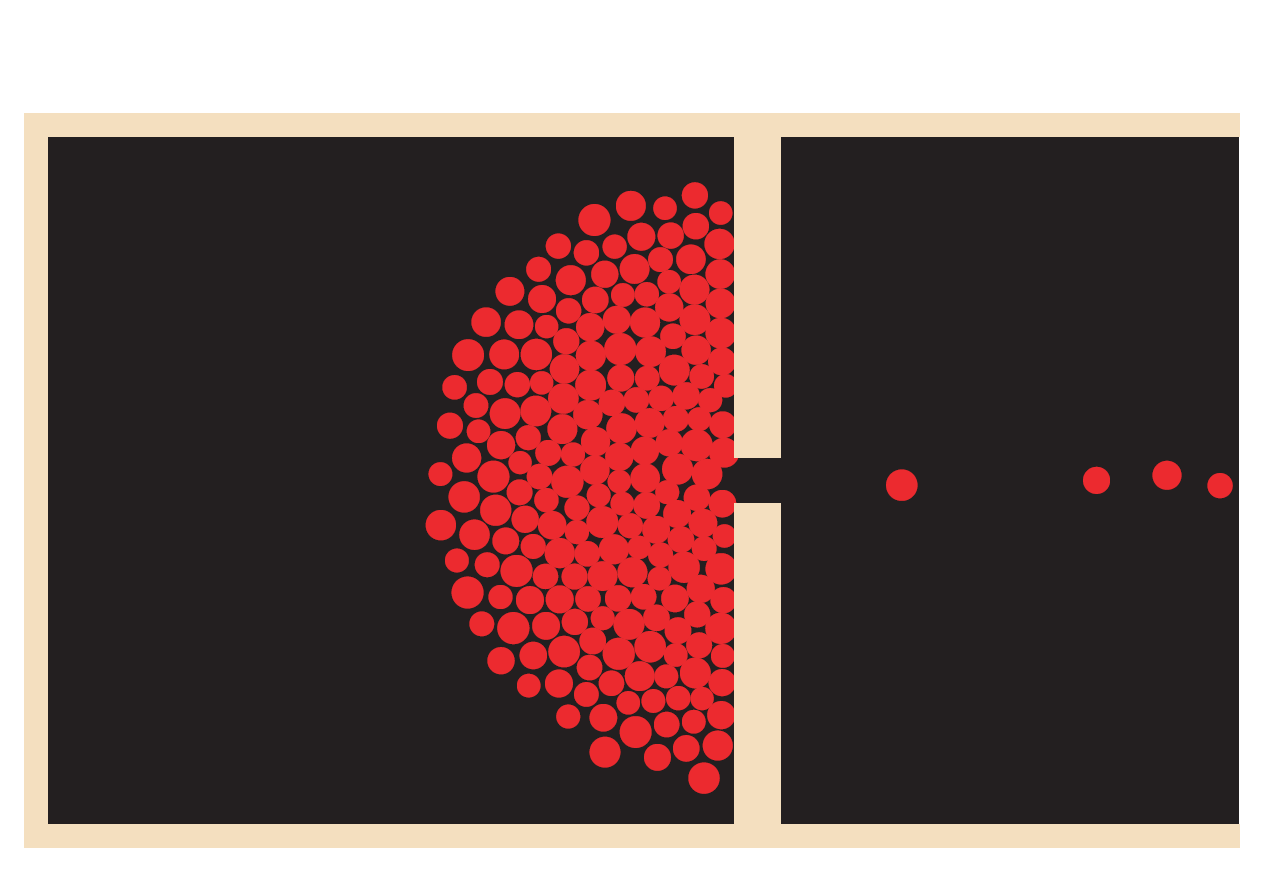
\includegraphics[width=0.45\textwidth]{Figures/square_room_letters.png}
        \label{subfig:fast-slow-clogging}
    }
    \subfloat[Leaving time versus desired velocity.]{
        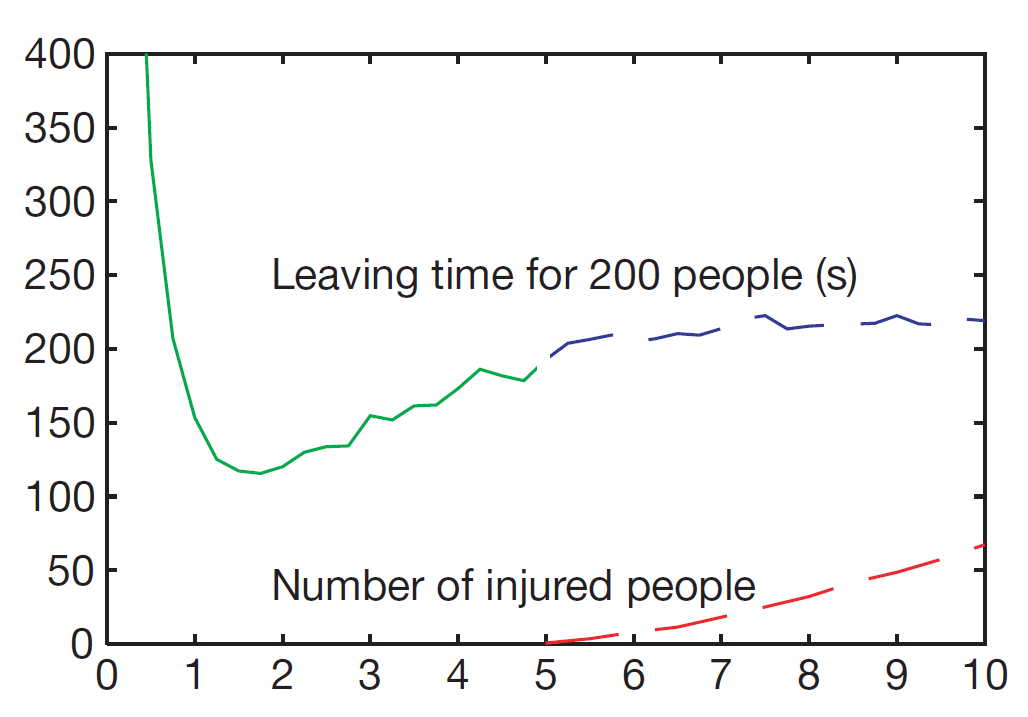
\includegraphics[width=0.45\textwidth]{Figures/leaving_time.png}
        \label{subfig:fast-slow-graph}
    }
    \caption[Faster-is-slower effect from \cite{helbing00}]{Faster-is-slower 
    effect from \cite{helbing00}. \subref{subfig:fast-slow-clogging} Clogging 
    occurs at doorways. \subref{subfig:fast-slow-graph} Fast desired 
    velocities leads to slower emptying of the room.}
    \label{fig:LtNFasterIsSlower}
\end{figure}

In our simulations of the square room scenario we have clogging in the 
doorways as expected (see figure~\ref{subfig:image-square-room}). 

In \cite{helbing00} they simulate a square room with dimensions 
$15\text{m} \cdot 15\text{m}$ with $200$ pedestrians as shown in 
figure \ref{fig:LtNFasterIsSlower}. In order to compare our results 
with theirs we simulate a corresponding scenario.

It has been necessary to lower the relaxation time of the pedestrians, $\tau$, 
from $1$ to $0.95$ when doing these simulation because with $\tau = 1$ the 
pedestrians would end up in a locked state in front of the door when there are 
three or four pedestrians left, where the repulsion between the pedestrians 
prevent either of them of passing through the doorway. With a lower value of 
$\tau$ this effect does not occur. 

It has also been necessary to remove the variation of the mean velocity when 
working at low velocities because some pedestrians ended up with an extremely 
low initial desired velocity which resulted in extremely high leaving times 
(for further discussion of this, see section~\ref{sec:random-errors}).

When we plot the time to leave the room as a function of the initial desired 
velocity with values from $0,75$ to $3,0$, as shown in 
figure~\ref{fig:square-room-leaving}, we do not see the leaving time increase 
with initial desired speed within any specific interval.  Looking at the 
results, we conclude that we do not see the faster-is-slower effect.

We choose to stop the initial desired speed at $3.0 \text{m}/\text{s}$ because 
if you increase it beyond this value people will start going through the walls 
and each other. One could avoid this by also increasing the wall potential and 
the strength of the social force, but such adjustments are not mentioned in 
the article. How they have managed to run model simulations with the initial 
desired velocity set to $10.0 \text{m}/\text{s}$ without seeing these errors 
is not clear.

\begin{figure}[ht]
    \centering
    \subfloat[Screen shot taken from the simulation]{
        \resizebox{0.35\textwidth}{!}{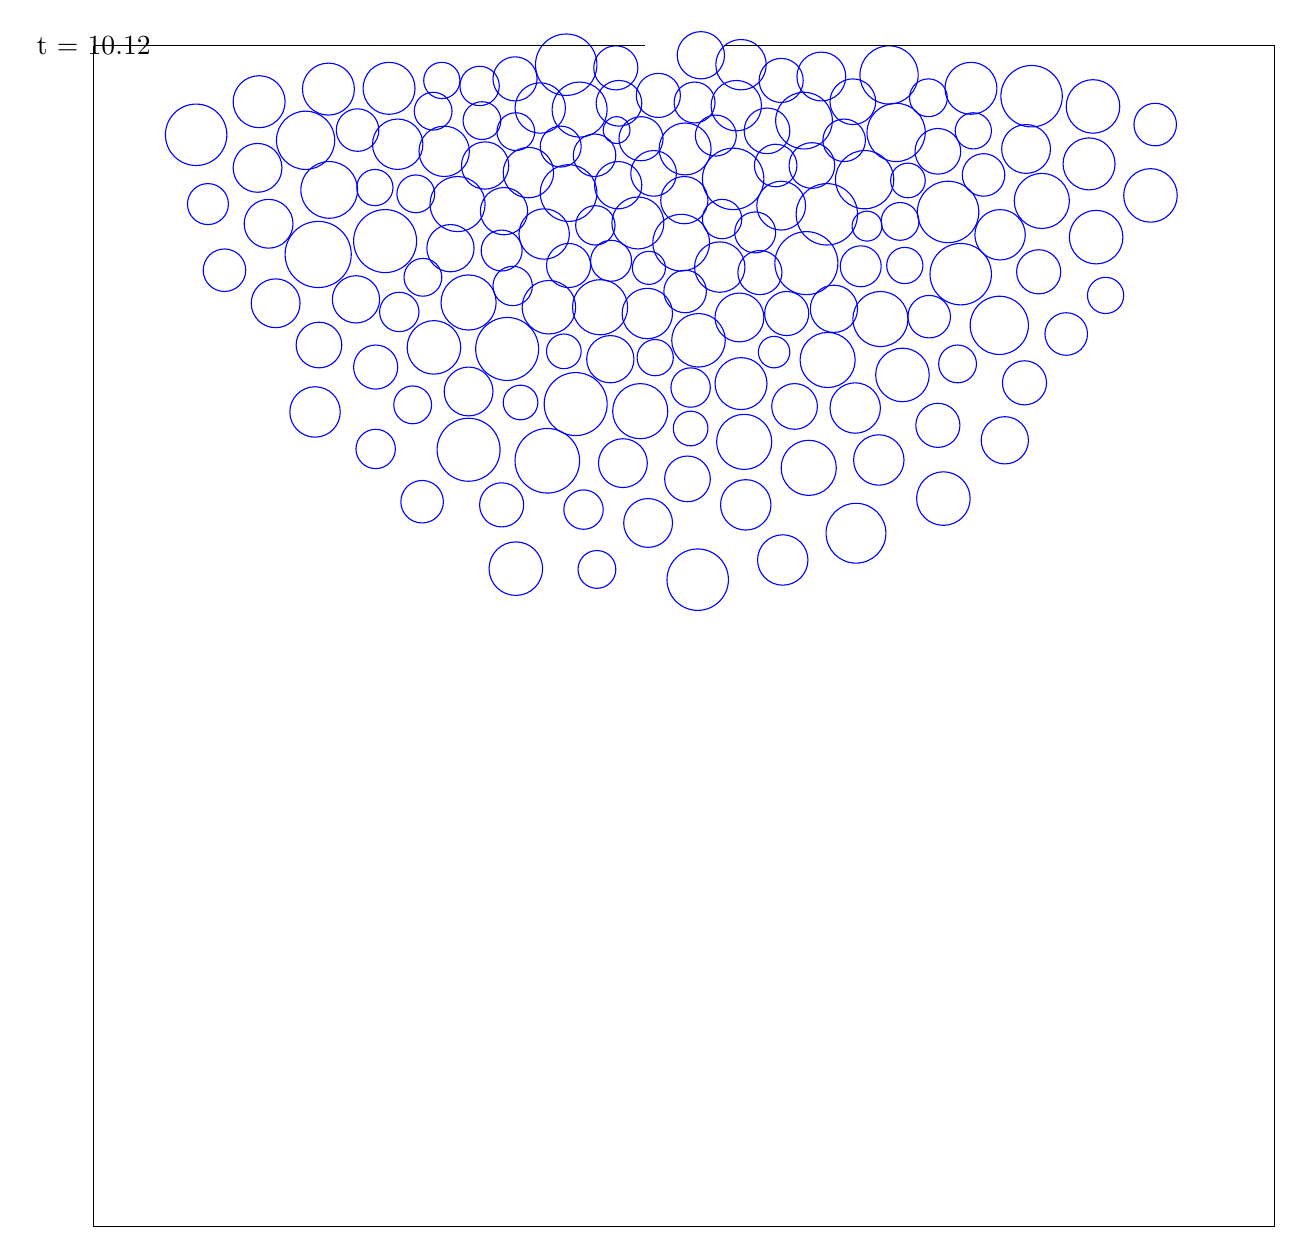
\begin{tikzpicture}
\draw[color=blue] (3.35,5.39) circle (0.39);
\draw[color=blue] (2.47,2.24) circle (0.32);
\draw[color=blue] (-1.74,2.23) circle (0.41);
\draw[color=blue] (0.17,0.72) circle (0.39);
\draw[color=blue] (-1.13,5.22) circle (0.25);
\draw[color=blue] (1.82,3.51) circle (0.35);
\draw[color=blue] (-0.83,6.77) circle (0.29);
\draw[color=blue] (-0.39,5.88) circle (0.29);
\draw[color=blue] (0.78,1.67) circle (0.32);
\draw[color=blue] (1.74,7.11) circle (0.31);
\draw[color=blue] (-1.72,4.18) circle (0.34);
\draw[color=blue] (1.23,5.47) circle (0.31);
\draw[color=blue] (0.45,4.69) circle (0.32);
\draw[color=blue] (-1.83,6.71) circle (0.32);
\draw[color=blue] (2.29,5.80) circle (0.37);
\draw[color=blue] (3.22,6.16) circle (0.29);
\draw[color=blue] (1.25,0.97) circle (0.32);
\draw[color=blue] (2.24,4.70) circle (0.26);
\draw[color=blue] (-0.86,6.43) circle (0.17);
\draw[color=blue] (2.77,3.32) circle (0.34);
\draw[color=blue] (-3.93,5.70) circle (0.23);
\draw[color=blue] (-0.94,3.52) circle (0.30);
\draw[color=blue] (2.18,1.31) circle (0.38);
\draw[color=blue] (2.69,6.40) circle (0.37);
\draw[color=blue] (2.17,2.90) circle (0.32);
\draw[color=blue] (-1.57,6.22) circle (0.26);
\draw[color=blue] (1.14,3.61) circle (0.20);
\draw[color=blue] (-5.19,4.23) circle (0.31);
\draw[color=blue] (-1.47,5.63) circle (0.36);
\draw[color=blue] (1.23,7.06) circle (0.28);
\draw[color=blue] (4.50,4.63) circle (0.28);
\draw[color=blue] (-3.92,2.38) circle (0.25);
\draw[color=blue] (3.67,6.42) circle (0.23);
\draw[color=blue] (-2.25,3.65) circle (0.40);
\draw[color=blue] (4.85,3.84) circle (0.27);
\draw[color=blue] (4.32,3.22) circle (0.28);
\draw[color=blue] (-3.41,5.62) circle (0.24);
\draw[color=blue] (5.23,5.07) circle (0.34);
\draw[color=blue] (-2.08,2.97) circle (0.22);
\draw[color=blue] (1.62,5.98) circle (0.29);
\draw[color=blue] (0.90,5.13) circle (0.26);
\draw[color=blue] (-3.33,1.71) circle (0.27);
\draw[color=blue] (-1.11,0.85) circle (0.24);
\draw[color=blue] (-0.84,5.73) circle (0.30);
\draw[color=blue] (0.66,6.74) circle (0.32);
\draw[color=blue] (-4.17,4.28) circle (0.30);
\draw[color=blue] (4.01,5.10) circle (0.32);
\draw[color=blue] (3.11,4.06) circle (0.27);
\draw[color=blue] (3.22,2.68) circle (0.28);
\draw[color=blue] (3.80,5.86) circle (0.27);
\draw[color=blue] (-0.33,6.87) circle (0.28);
\draw[color=blue] (-0.45,4.68) circle (0.21);
\draw[color=blue] (-0.46,1.44) circle (0.31);
\draw[color=blue] (-1.47,4.71) circle (0.28);
\draw[color=blue] (0.08,2.64) circle (0.22);
\draw[color=blue] (-1.98,5.89) circle (0.32);
\draw[color=blue] (-2.97,4.93) circle (0.30);
\draw[color=blue] (-3.18,3.67) circle (0.34);
\draw[color=blue] (-2.74,3.11) circle (0.31);
\draw[color=blue] (-1.78,5.11) circle (0.32);
\draw[color=blue] (2.03,6.30) circle (0.27);
\draw[color=blue] (0.96,4.62) circle (0.28);
\draw[color=blue] (4.07,2.49) circle (0.30);
\draw[color=blue] (3.47,3.46) circle (0.24);
\draw[color=blue] (0.76,2.47) circle (0.35);
\draw[color=blue] (-1.53,3.62) circle (0.22);
\draw[color=blue] (2.60,7.13) circle (0.37);
\draw[color=blue] (-1.50,7.26) circle (0.39);
\draw[color=blue] (0.48,5.30) circle (0.25);
\draw[color=blue] (-0.56,2.86) circle (0.35);
\draw[color=blue] (4.34,6.19) circle (0.31);
\draw[color=blue] (2.49,4.03) circle (0.35);
\draw[color=blue] (0.18,3.76) circle (0.34);
\draw[color=blue] (-6.20,6.37) circle (0.39);
\draw[color=blue] (-0.78,2.20) circle (0.31);
\draw[color=blue] (0.62,5.81) circle (0.39);
\draw[color=blue] (-0.37,3.54) circle (0.23);
\draw[color=blue] (-3.32,4.56) circle (0.24);
\draw[color=blue] (-3.45,2.94) circle (0.24);
\draw[color=blue] (-2.74,2.37) circle (0.40);
\draw[color=blue] (-0.55,6.32) circle (0.28);
\draw[color=blue] (1.55,4.74) circle (0.40);
\draw[color=blue] (-4.81,6.30) circle (0.37);
\draw[color=blue] (1.81,5.36) circle (0.39);
\draw[color=blue] (4.54,5.53) circle (0.35);
\draw[color=blue] (-6.05,5.49) circle (0.26);
\draw[color=blue] (-1.38,2.95) circle (0.40);
\draw[color=blue] (0.04,2.00) circle (0.29);
\draw[color=blue] (5.92,5.60) circle (0.34);
\draw[color=blue] (1.58,2.14) circle (0.35);
\draw[color=blue] (2.14,6.79) circle (0.29);
\draw[color=blue] (3.64,6.96) circle (0.33);
\draw[color=blue] (-1.07,4.18) circle (0.35);
\draw[color=blue] (-2.18,4.45) circle (0.25);
\draw[color=blue] (0.70,4.05) circle (0.31);
\draw[color=blue] (-5.84,4.65) circle (0.27);
\draw[color=blue] (-4.64,3.70) circle (0.29);
\draw[color=blue] (3.51,4.60) circle (0.39);
\draw[color=blue] (-5.40,6.79) circle (0.33);
\draw[color=blue] (-3.64,6.25) circle (0.32);
\draw[color=blue] (-0.93,4.77) circle (0.26);
\draw[color=blue] (-0.59,5.25) circle (0.33);
\draw[color=blue] (0.01,4.38) circle (0.27);
\draw[color=blue] (0.00,5.54) circle (0.30);
\draw[color=blue] (-4.15,6.43) circle (0.27);
\draw[color=blue] (-4.52,6.95) circle (0.33);
\draw[color=blue] (5.14,6.00) circle (0.33);
\draw[color=blue] (1.40,2.92) circle (0.29);
\draw[color=blue] (-3.05,6.16) circle (0.32);
\draw[color=blue] (0.08,3.16) circle (0.25);
\draw[color=blue] (5.35,4.33) circle (0.23);
\draw[color=blue] (-0.47,4.10) circle (0.32);
\draw[color=blue] (-5.42,5.95) circle (0.31);
\draw[color=blue] (0.01,6.19) circle (0.33);
\draw[color=blue] (-4.65,4.85) circle (0.42);
\draw[color=blue] (-2.88,5.49) circle (0.35);
\draw[color=blue] (-1.28,1.61) circle (0.25);
\draw[color=blue] (1.52,6.55) circle (0.36);
\draw[color=blue] (2.80,4.71) circle (0.23);
\draw[color=blue] (-3.92,3.42) circle (0.28);
\draw[color=blue] (-2.29,5.40) circle (0.30);
\draw[color=blue] (4.41,6.86) circle (0.39);
\draw[color=blue] (0.40,6.36) circle (0.26);
\draw[color=blue] (-2.32,4.90) circle (0.26);
\draw[color=blue] (1.90,4.16) circle (0.30);
\draw[color=blue] (1.16,5.98) circle (0.27);
\draw[color=blue] (-4.51,5.67) circle (0.36);
\draw[color=blue] (-2.60,6.99) circle (0.25);
\draw[color=blue] (-2.57,6.55) circle (0.24);
\draw[color=blue] (1.30,4.10) circle (0.28);
\draw[color=blue] (-2.15,7.08) circle (0.28);
\draw[color=blue] (-3.80,5.02) circle (0.40);
\draw[color=blue] (-2.74,4.24) circle (0.35);
\draw[color=blue] (0.21,7.38) circle (0.30);
\draw[color=blue] (-3.19,6.67) circle (0.24);
\draw[color=blue] (-2.14,0.86) circle (0.34);
\draw[color=blue] (2.84,5.79) circle (0.22);
\draw[color=blue] (-0.04,5.00) circle (0.36);
\draw[color=blue] (-4.69,2.85) circle (0.32);
\draw[color=blue] (-1.33,6.69) circle (0.35);
\draw[color=blue] (0.72,7.26) circle (0.32);
\draw[color=blue] (5.98,6.50) circle (0.27);
\draw[color=blue] (-3.62,4.12) circle (0.25);
\draw[color=blue] (-1.14,6.11) circle (0.27);
\draw[color=blue] (-0.87,7.22) circle (0.28);
\draw[color=blue] (-2.32,1.67) circle (0.28);
\draw[color=blue] (-3.08,7.06) circle (0.23);
\draw[color=blue] (2.32,5.21) circle (0.19);
\draw[color=blue] (-3.75,6.96) circle (0.33);
\draw[color=blue] (2.74,5.27) circle (0.24);
\draw[color=blue] (0.13,6.78) circle (0.26);
\draw[color=blue] (-2.14,6.41) circle (0.24);
\draw[color=blue] (-5.28,5.24) circle (0.31);
\draw[color=blue] (-2.53,5.98) circle (0.30);
\draw[color=blue] (3.10,6.84) circle (0.24);
\draw[color=blue] (0.72,3.21) circle (0.33);
\draw[color=blue] (1.05,6.42) circle (0.29);
\draw[color=blue] (5.19,6.73) circle (0.34);
\draw[color=blue] (3.29,1.75) circle (0.34);
\draw[color=blue] (4.00,3.95) circle (0.37);
\node at (-7.50, 7.50) {t = 10.12};
\useasboundingbox (-7.50, -7.50) rectangle (7.50, 7.50);
\draw[color=black] (-7.50,-7.50) -- (7.50,-7.50);
\draw[color=black] (-7.50,-7.50) -- (-7.50,7.50);
\draw[color=black] (7.50,-7.50) -- (7.50,7.50);
\draw[color=black] (7.50,7.50) -- (0.50,7.50);
\draw[color=black] (-7.50,7.50) -- (-0.50,7.50);
\end{tikzpicture}
}
    }
    \subfloat[Time to clear the room as a function of mean desired velocity.]{
        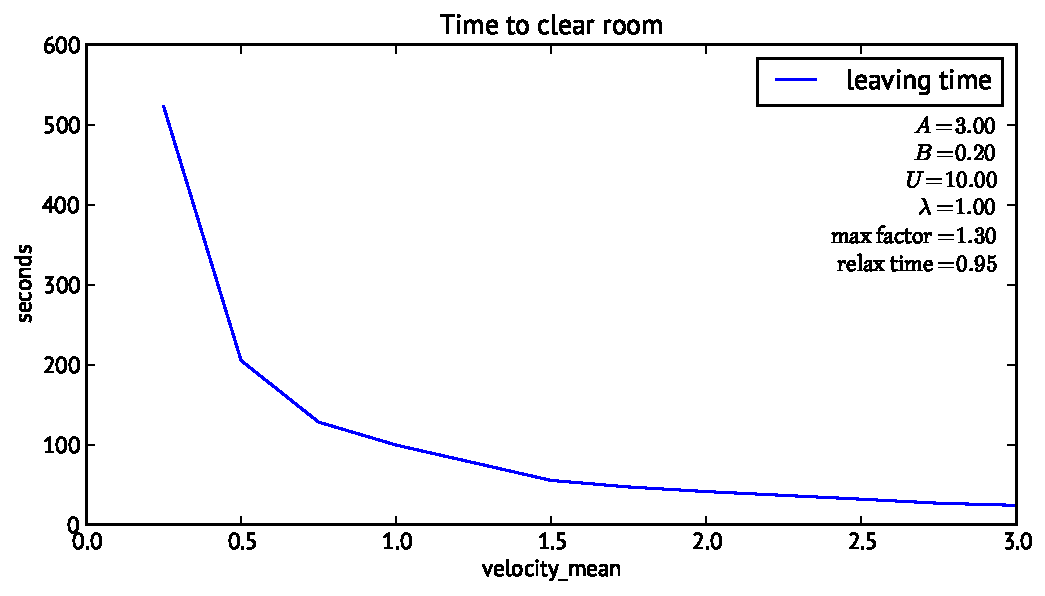
\includegraphics[width=0.65\textwidth]{Figures/time-to-clear.pdf}
    }
    \caption[Leaving time for the square room]{Leaving time for the square 
    room. We do not see the increase in leaving time as we increase the 
    initial desired speed.}
    \label{fig:square-room-leaving}
\end{figure}

\subsubsection{Lane formation}
Lane formation happens when the simulation contains bidirectional flow in 
corridors. As stated in \ref{self-org}:

\begin{quote}
    If pedestrians crowds moving in opposite directions meet each other, they 
    form small \emph{channels} in the beginning, but these channels later 
    merge to produce wide lanes
\end{quote}

An illustration of this phenomenon from \cite{lanes} can be seen in 
figure~\ref{fig:lanes-literature}. 

\begin{figure}[h]
    \centering
    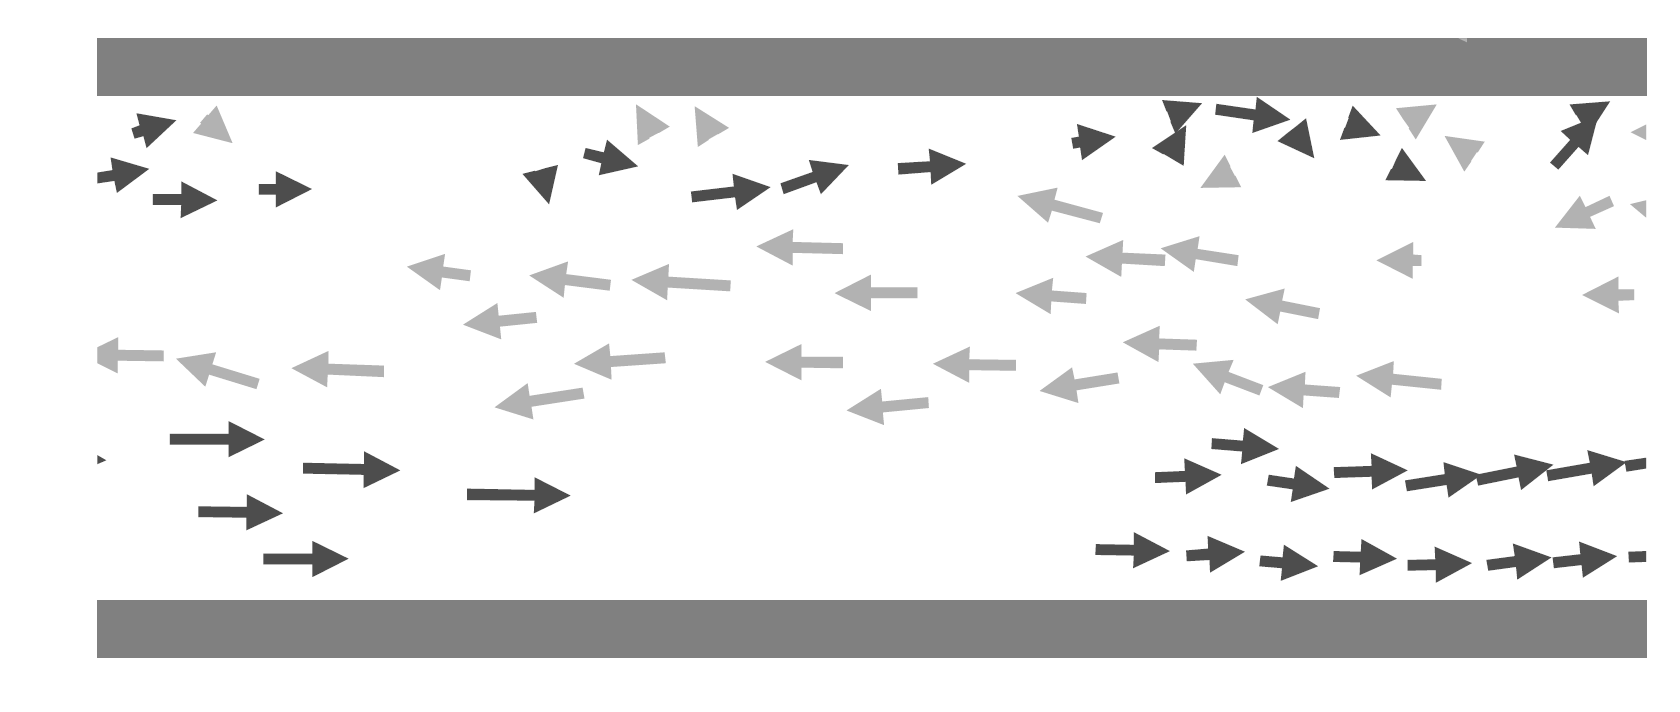
\includegraphics[width=0.8\textwidth]{Figures/flow_lanes_litterature.png}
    \caption[Lane formation from \cite{lanes}]{Lane formation from 
    \cite{lanes}. Pedestrians through a corridor form alternating lanes of 
    pedestrians going in each direction.}
    \label{fig:lanes-literature}
\end{figure}

Since we have two different corridor cases we have looked for lane
formation in both of them. As can be seen in figure~\ref{fig:laneformation}, 
the lane formation occurs in both cases.

\begin{figure}[h]
    \centering
    \subfloat[Bidirectional flow in a corridor.]{
        \resizebox{0.45\textwidth}{!}{\begin{tikzpicture}
\draw[color=blue] (-2.64,-1.02) circle (0.34);
\draw[color=blue] (-2.89,0.96) circle (0.31);
\draw[color=green] (5.10,-0.19) circle (0.32);
\draw[color=green] (2.19,0.17) circle (0.34);
\draw[color=green] (7.16,-1.49) circle (0.34);
\draw[color=green] (4.10,0.13) circle (0.28);
\draw[color=blue] (-5.87,0.58) circle (0.32);
\draw[color=green] (4.72,-1.57) circle (0.30);
\draw[color=blue] (-0.53,1.69) circle (0.30);
\draw[color=blue] (-2.13,1.68) circle (0.31);
\draw[color=blue] (-5.04,-0.15) circle (0.30);
\draw[color=green] (5.64,-1.69) circle (0.33);
\draw[color=green] (3.38,-1.57) circle (0.32);
\draw[color=blue] (-10.87,-1.75) circle (0.30);
\draw[color=green] (6.43,-0.42) circle (0.31);
\draw[color=green] (2.34,-1.60) circle (0.31);
\draw[color=blue] (-4.76,1.74) circle (0.33);
\draw[color=blue] (-8.66,1.76) circle (0.30);
\draw[color=blue] (-9.81,1.46) circle (0.31);
\draw[color=blue] (-3.52,1.75) circle (0.28);
\draw[color=blue] (-1.27,1.16) circle (0.25);
\draw[color=blue] (-2.06,0.63) circle (0.31);
\draw[color=green] (7.84,-1.70) circle (0.32);
\draw[color=blue] (-1.27,-0.56) circle (0.29);
\draw[color=blue] (-0.27,-0.60) circle (0.35);
\draw[color=green] (1.33,-1.66) circle (0.27);
\draw[color=green] (0.99,0.39) circle (0.30);
\draw[color=blue] (1.08,-0.61) circle (0.30);
\draw[color=blue] (-4.23,-0.62) circle (0.33);
\draw[color=blue] (-6.83,1.76) circle (0.33);
\draw[color=blue] (2.23,1.76) circle (0.29);
\draw[color=blue] (0.34,1.27) circle (0.28);
\draw[color=blue] (1.12,1.73) circle (0.30);
\draw[color=green] (-1.39,-0.16) circle (0.27);
\draw[color=green] (0.26,-1.60) circle (0.28);
\draw[color=green] (-3.13,0.14) circle (0.31);
\draw[color=blue] (5.12,-0.87) circle (0.32);
\draw[color=blue] (2.68,-0.64) circle (0.31);
\draw[color=blue] (4.72,1.61) circle (0.28);
\draw[color=green] (-0.92,-1.72) circle (0.29);
\draw[color=blue] (1.78,0.88) circle (0.28);
\draw[color=blue] (3.41,1.80) circle (0.31);
\draw[color=blue] (3.57,1.05) circle (0.33);
\draw[color=green] (-3.73,0.67) circle (0.32);
\draw[color=green] (-3.21,-1.68) circle (0.28);
\draw[color=green] (-4.56,-1.74) circle (0.29);
\draw[color=green] (-2.18,-1.73) circle (0.30);
\draw[color=green] (-6.02,-0.90) circle (0.31);
\draw[color=green] (-5.41,-0.54) circle (0.30);
\draw[color=blue] (8.22,-1.63) circle (0.30);
\draw[color=blue] (6.29,1.33) circle (0.34);
\draw[color=blue] (5.78,0.55) circle (0.27);
\draw[color=green] (-6.35,0.65) circle (0.28);
\draw[color=green] (-9.00,-1.11) circle (0.29);
\draw[color=blue] (6.83,-0.45) circle (0.34);
\draw[color=green] (-7.61,0.21) circle (0.34);
\draw[color=blue] (7.83,0.76) circle (0.28);
\draw[color=green] (-7.85,-1.11) circle (0.29);
\draw[color=green] (-9.23,0.34) circle (0.32);
\draw[color=green] (-8.66,-0.31) circle (0.31);
%\node at (-12.50, 5.83) {t = 10.12};
\useasboundingbox (-12.50, -5.83) rectangle (12.50, 5.83);
\draw[color=black] (-10.00,2.50) -- (10.00,2.50);
\draw[color=black] (-10.00,-2.50) -- (10.00,-2.50);
\end{tikzpicture}
}
    }
    \subfloat[Bidirectional flow in a corridor with a bottleneck.]{
        \resizebox{0.45\textwidth}{!}{\begin{tikzpicture}
\draw[color=blue] (-5.03,-1.14) circle (0.32);
\draw[color=blue] (-8.18,-1.13) circle (0.29);
\draw[color=blue] (-12.00,-0.90) circle (0.29);
\draw[color=blue] (-11.43,-1.43) circle (0.28);
\draw[color=blue] (-7.50,-0.61) circle (0.29);
\draw[color=blue] (-10.95,-0.73) circle (0.30);
\draw[color=blue] (-6.99,-1.13) circle (0.29);
\draw[color=blue] (-8.55,0.46) circle (0.29);
\draw[color=blue] (-3.37,-0.90) circle (0.29);
\draw[color=blue] (-6.46,0.83) circle (0.30);
\draw[color=green] (9.68,-0.09) circle (0.28);
\draw[color=green] (7.24,0.24) circle (0.29);
\draw[color=green] (8.09,-0.29) circle (0.31);
\draw[color=blue] (-1.95,0.74) circle (0.31);
\draw[color=blue] (-2.91,-0.60) circle (0.30);
\draw[color=blue] (-4.56,0.81) circle (0.29);
\draw[color=green] (6.58,-0.35) circle (0.30);
\draw[color=blue] (-6.57,-0.54) circle (0.29);
\draw[color=blue] (0.40,0.19) circle (0.30);
\draw[color=blue] (-8.24,1.03) circle (0.31);
\draw[color=green] (4.36,0.09) circle (0.31);
\draw[color=green] (5.12,-0.62) circle (0.29);
\draw[color=green] (6.32,0.45) circle (0.30);
\draw[color=green] (4.08,0.79) circle (0.30);
\draw[color=green] (3.85,-0.67) circle (0.30);
\draw[color=green] (5.71,-0.05) circle (0.30);
\draw[color=blue] (-1.45,0.19) circle (0.30);
\draw[color=blue] (1.44,-0.95) circle (0.32);
\draw[color=blue] (-2.38,-0.55) circle (0.29);
\draw[color=green] (3.56,0.11) circle (0.29);
\draw[color=green] (-1.76,0.10) circle (0.30);
\draw[color=blue] (-1.85,-0.67) circle (0.32);
\draw[color=green] (0.28,0.64) circle (0.32);
\draw[color=blue] (-1.22,-0.43) circle (0.29);
\draw[color=green] (-0.38,0.74) circle (0.30);
\draw[color=green] (-2.27,0.27) circle (0.31);
\draw[color=green] (-1.10,1.07) circle (0.31);
\draw[color=blue] (4.11,-1.40) circle (0.30);
\draw[color=green] (-1.88,1.32) circle (0.30);
\draw[color=green] (-3.72,-1.86) circle (0.29);
\draw[color=green] (-2.67,0.05) circle (0.30);
\draw[color=blue] (3.92,1.40) circle (0.31);
\draw[color=green] (-4.24,1.75) circle (0.29);
\draw[color=blue] (5.16,-1.32) circle (0.29);
\draw[color=green] (-5.12,0.08) circle (0.29);
\draw[color=green] (-6.04,1.97) circle (0.31);
\draw[color=blue] (7.08,1.47) circle (0.30);
\draw[color=green] (-6.81,2.11) circle (0.29);
\draw[color=blue] (7.23,0.72) circle (0.30);
\draw[color=blue] (7.43,-1.11) circle (0.32);
\draw[color=blue] (7.91,2.22) circle (0.29);
\draw[color=green] (-8.85,0.66) circle (0.29);
\draw[color=green] (-8.91,-2.45) circle (0.30);
\draw[color=green] (-9.52,-1.90) circle (0.29);
%\node at (-12.50, 5.83) {t = 18.99};
\useasboundingbox (-12.50, -5.83) rectangle (12.50, 5.83);
\draw[color=black] (-10.00,3.00) -- (-5.00,3.00);
\draw[color=black] (-10.00,-3.00) -- (-5.00,-3.00);
\draw[color=black] (-5.00,3.00) -- (0.00,1.00);
\draw[color=black] (-5.00,-3.00) -- (0.00,-1.00);
\draw[color=black] (0.00,1.00) -- (5.00,3.00);
\draw[color=black] (0.00,-1.00) -- (5.00,-3.00);
\draw[color=black] (5.00,3.00) -- (10.00,3.00);
\draw[color=black] (5.00,-3.00) -- (10.00,-3.00);
\end{tikzpicture}
}
    }
    \caption[Lane formation in corridor simulations]{Lane formation in 
    corridor simulations. The colours indicate the direction the pedestrians 
    are moving in. The blue ones are walking to the left; the green ones are 
    walking to the right. Lane formation can be seen in both cases. }
    \label{fig:laneformation}
\end{figure}

\subsubsection{Freezing by heating effect}
The freezing by heating effect occurs when the lane formations break down due 
to extreme densities. This results in a clogging that brings the pedestrians 
to a complete halt (see section~\ref{sec:article-results}).  The illustration 
of this effect as presented in \cite{oscil} can be seen in 
figure~\ref{fig:freezing_by_heating_litterature}.

\begin{figure}[h]
    \centering
    \subfloat[Freezing by heating effect from \cite{oscil}.]{
        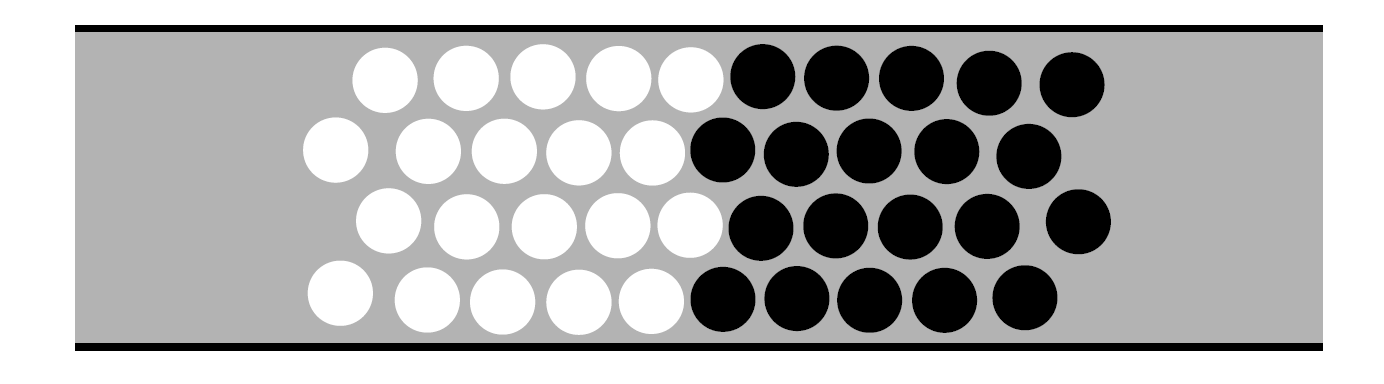
\includegraphics[width=0.45\textwidth]{Figures/heatfreeze.png}
    }
    \subfloat[Freezing-by-heating effect from our simulation.]{
        \resizebox{0.45\textwidth}{!}{\begin{tikzpicture}
\draw[color=blue] (-4.00,-0.49) circle (0.39);
\draw[color=green] (4.39,-1.05) circle (0.35);
\draw[color=blue] (0.51,1.24) circle (0.39);
\draw[color=blue] (-2.15,-0.86) circle (0.35);
\draw[color=green] (1.75,-0.77) circle (0.29);
\draw[color=green] (3.79,-1.00) circle (0.31);
\draw[color=blue] (-1.69,-1.17) circle (0.34);
\draw[color=blue] (-3.31,-0.10) circle (0.32);
\draw[color=green] (-0.23,1.26) circle (0.37);
\draw[color=blue] (-0.82,0.18) circle (0.32);
\draw[color=green] (1.44,-0.49) circle (0.17);
\draw[color=blue] (1.26,0.45) circle (0.34);
\draw[color=blue] (-2.61,0.71) circle (0.41);
\draw[color=blue] (-0.30,0.12) circle (0.30);
\draw[color=blue] (-3.46,0.73) circle (0.38);
\draw[color=blue] (0.53,0.54) circle (0.31);
\draw[color=green] (0.97,-0.77) circle (0.26);
\draw[color=green] (-0.93,1.14) circle (0.28);
\draw[color=blue] (-1.01,-1.23) circle (0.36);
\draw[color=blue] (-0.02,0.66) circle (0.28);
\draw[color=blue] (2.01,-1.16) circle (0.25);
\draw[color=blue] (-4.98,0.43) circle (0.21);
\draw[color=blue] (0.17,0.01) circle (0.27);
\draw[color=green] (1.28,-1.14) circle (0.24);
\draw[color=blue] (-0.73,-0.76) circle (0.22);
\draw[color=green] (-0.52,0.71) circle (0.26);
\draw[color=blue] (4.82,-0.91) circle (0.27);
\draw[color=blue] (0.67,-0.04) circle (0.30);
\draw[color=blue] (-0.13,-1.13) circle (0.30);
\draw[color=blue] (2.71,-1.18) circle (0.27);
\draw[color=blue] (1.94,0.83) circle (0.27);
\draw[color=blue] (1.03,0.93) circle (0.26);
\draw[color=blue] (2.09,-0.44) circle (0.31);
\draw[color=green] (-2.85,1.17) circle (0.22);
\draw[color=green] (0.54,-0.66) circle (0.25);
\draw[color=green] (-1.71,1.11) circle (0.34);
\draw[color=blue] (2.66,-0.45) circle (0.36);
\draw[color=blue] (1.53,1.16) circle (0.32);
\draw[color=blue] (2.40,0.64) circle (0.26);
\draw[color=green] (0.05,-0.60) circle (0.28);
\draw[color=blue] (1.16,-0.14) circle (0.24);
\draw[color=blue] (1.76,0.14) circle (0.32);
\draw[color=blue] (3.99,1.00) circle (0.37);
\draw[color=green] (-1.87,0.40) circle (0.36);
\draw[color=green] (-2.51,-0.44) circle (0.25);
\draw[color=green] (-0.38,-0.39) circle (0.28);
\draw[color=green] (-1.30,0.08) circle (0.31);
\draw[color=green] (-2.58,0.08) circle (0.32);
\draw[color=green] (-1.19,0.68) circle (0.30);
\draw[color=blue] (3.33,-0.51) circle (0.31);
\draw[color=blue] (2.63,1.25) circle (0.39);
\draw[color=blue] (2.90,0.66) circle (0.24);
\draw[color=green] (-3.71,0.20) circle (0.24);
\draw[color=green] (-4.41,-0.99) circle (0.28);
\draw[color=blue] (3.07,0.09) circle (0.40);
\draw[color=green] (-1.23,-0.54) circle (0.39);
\draw[color=blue] (2.29,0.18) circle (0.26);
\draw[color=green] (-1.87,-0.25) circle (0.29);
\draw[color=green] (-5.34,0.02) circle (0.35);
\draw[color=green] (-2.69,-1.11) circle (0.33);
\draw[color=blue] (4.08,-0.30) circle (0.32);
\draw[color=green] (-3.89,1.13) circle (0.31);
\draw[color=green] (-3.59,-1.12) circle (0.27);
\draw[color=green] (-4.50,-0.11) circle (0.28);
\draw[color=blue] (3.73,0.29) circle (0.33);
\draw[color=green] (-4.26,0.39) circle (0.26);
\draw[color=blue] (3.35,0.95) circle (0.27);
\draw[color=green] (-4.94,-0.62) circle (0.27);
\draw[color=green] (-3.17,-0.71) circle (0.33);
\draw[color=blue] (7.92,0.49) circle (0.32);
\draw[color=green] (-4.53,0.89) circle (0.23);
\draw[color=blue] (4.69,-0.10) circle (0.31);
\draw[color=blue] (5.33,-0.57) circle (0.42);
\draw[color=blue] (4.76,0.98) circle (0.25);
\draw[color=green] (-5.20,0.88) circle (0.23);
\draw[color=green] (-5.38,-0.92) circle (0.30);
\draw[color=green] (-5.67,1.02) circle (0.26);
\draw[color=blue] (6.07,-0.90) circle (0.30);
\draw[color=green] (-6.07,0.07) circle (0.36);
\draw[color=green] (-6.15,0.89) circle (0.24);
\draw[color=blue] (4.43,0.46) circle (0.28);
\draw[color=blue] (5.64,0.17) circle (0.35);
\draw[color=blue] (6.41,-0.34) circle (0.24);
\draw[color=green] (-9.99,-0.79) circle (0.25);
\draw[color=blue] (8.05,-0.55) circle (0.36);
\draw[color=green] (-6.05,-0.93) circle (0.35);
\draw[color=blue] (5.47,0.89) circle (0.34);
\draw[color=blue] (6.22,0.67) circle (0.25);
\draw[color=green] (-6.70,-0.75) circle (0.26);
\draw[color=green] (-9.22,0.75) circle (0.28);
\draw[color=blue] (7.08,-0.24) circle (0.28);
\draw[color=green] (-8.95,-0.37) circle (0.27);
\draw[color=green] (-6.69,0.39) circle (0.33);
\draw[color=green] (-6.81,0.94) circle (0.24);
\draw[color=green] (-8.33,-0.92) circle (0.26);
\draw[color=green] (-9.79,0.20) circle (0.24);
\draw[color=green] (-7.20,-0.15) circle (0.30);
\draw[color=green] (-8.26,1.07) circle (0.33);
\draw[color=green] (-7.37,-1.00) circle (0.34);
\draw[color=green] (-7.95,-0.34) circle (0.41);
\draw[color=blue] (9.46,0.01) circle (0.28);
\draw[color=green] (-8.54,0.48) circle (0.35);
\draw[color=green] (-9.48,-0.37) circle (0.33);
\node at (-12.50, 5.83) {t = 20.55};
\useasboundingbox (-12.50, -5.83) rectangle (12.50, 5.83);
\draw[color=black] (-10.00,1.50) -- (10.00,1.50);
\draw[color=black] (-10.00,-1.50) -- (10.00,-1.50);
\end{tikzpicture}
}
    }
    \caption[Freezing-by-heating effect from \cite{oscil} compared with our 
    own.]{Freezing-by-heating effect from \cite{oscil} compared with our own.}
    \label{fig:freezing_by_heating_litterature}
\end{figure}

We have been able to reproduce the freezing-by-heating effect in both corridor 
cases. Actually, in most cases run with a high density of pedestrians, we see 
the effect in our simulations.  

\subsubsection{Oscillating flows}
Oscillating flows occur when clogging occurs at a bottleneck, and small groups 
of pedestrians from each direction alternate in getting through the 
bottleneck. The effect is described in \cite{oscil}, but it is not clear how 
they measure it. Figure~\ref{fig:oscillitoryflow_litterature} shows the 
illustration from the article that explains the effect.

When looking at the simulation, it is apparent that clogging appears in both 
ends of the bottleneck and people are sometimes squeezed through the 
bottleneck, but it is not immediately clear whether this constitutes an 
oscillating flow.  To get a better indication of whether or not oscillation 
occurs, we have graphed the flow rate in each direction. This graph is seen in 
figure~\ref{fig:oscillatory-flow}. The graph does not show a clear indication 
of oscillating flows, however a possible source of error is that the flow rate 
is measured at the ends of the corridor, which may dilute the effect as 
pedestrians are passing through the crowd after having passed through the 
bottleneck. However, in the way our simulation is implemented, it is not 
possible to distinguish between pedestrians moving in different directions 
when measuring the flow rate in the middle of the bottleneck.

In conclusion, we may be able to replicate the oscillating flows, but the 
results are not completely clear.

\begin{figure}[h]
    \centering
    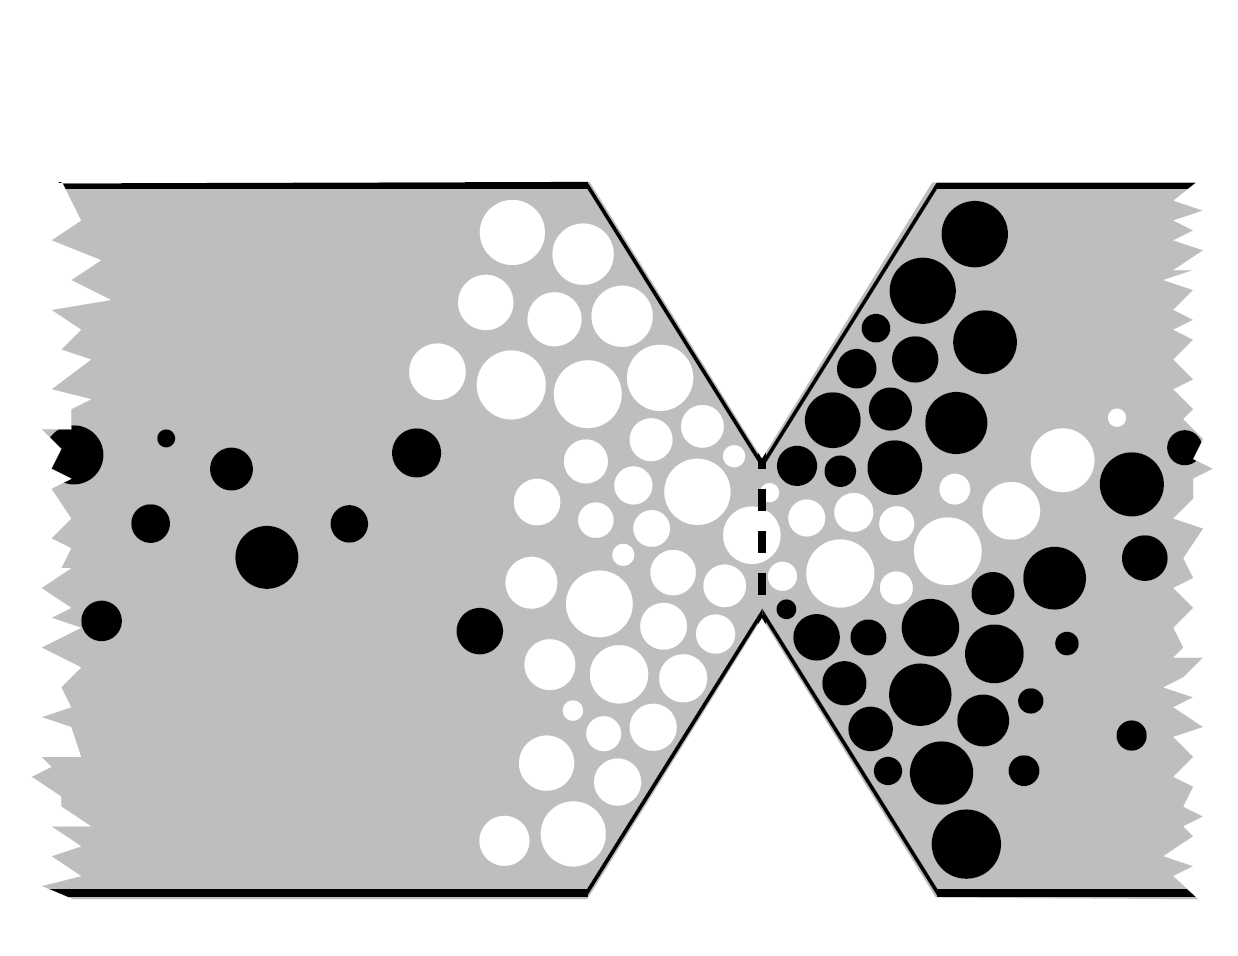
\includegraphics[width=0.4\textwidth]{Figures/oscil_flow.png}
    \caption[Illustration of oscillating flow from \cite{oscil}]{Illustration 
    of oscillating flow from \cite{oscil}. A small group of pedestrians 
    slipping through the bottleneck passes through the bottleneck in one 
    direction. Oscillations occur when pedestrians alternately pass through 
    the bottleneck from each direction.}
    \label{fig:oscillitoryflow_litterature}
\end{figure}

\begin{figure}[h]
    \centering
    \subfloat[Flowrates measured at each end of the corridor]{
        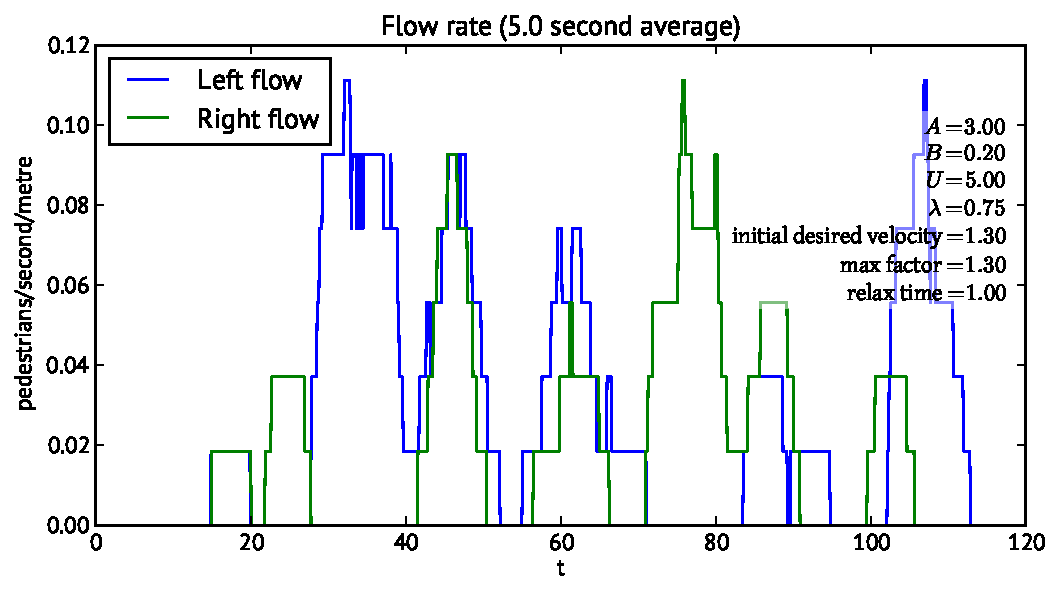
\includegraphics[width=0.45\textwidth]{Figures/flowrateBiDirecBottle.pdf}
        \label{subfig:flow-graph}
    }
    \subfloat[Clogging of a bottleneck]{
        \resizebox{0.45\textwidth}{!}{\begin{tikzpicture}
\draw[color=green] (-1.76,-0.12) circle (0.30);
\draw[color=blue] (0.64,-0.77) circle (0.30);
\draw[color=blue] (0.10,0.27) circle (0.30);
\draw[color=green] (-0.37,-0.03) circle (0.30);
\draw[color=blue] (1.17,0.92) circle (0.30);
\draw[color=blue] (1.87,-0.30) circle (0.30);
\draw[color=blue] (0.55,0.67) circle (0.30);
\draw[color=blue] (1.64,0.42) circle (0.30);
\draw[color=blue] (-4.68,-1.58) circle (0.30);
\draw[color=green] (1.32,-0.23) circle (0.30);
\draw[color=green] (0.85,0.04) circle (0.30);
\draw[color=green] (-0.52,-0.70) circle (0.30);
\draw[color=green] (-0.40,0.73) circle (0.30);
\draw[color=green] (-1.35,-0.68) circle (0.30);
\draw[color=green] (0.30,-0.35) circle (0.30);
\draw[color=blue] (1.97,1.10) circle (0.30);
\draw[color=blue] (1.34,-0.95) circle (0.30);
\draw[color=blue] (2.46,0.40) circle (0.30);
\draw[color=green] (-0.97,0.21) circle (0.30);
\draw[color=green] (-2.66,0.11) circle (0.30);
\draw[color=blue] (2.50,-0.53) circle (0.30);
\draw[color=green] (-1.35,0.87) circle (0.30);
\draw[color=blue] (1.97,-1.16) circle (0.30);
\draw[color=green] (-1.99,0.89) circle (0.30);
\draw[color=green] (-4.08,-0.52) circle (0.30);
\draw[color=green] (-3.93,0.62) circle (0.30);
\draw[color=blue] (7.18,-1.19) circle (0.30);
\draw[color=green] (-7.18,1.24) circle (0.30);
\draw[color=green] (-8.93,-1.69) circle (0.30);
\draw[color=green] (-9.49,-0.01) circle (0.30);
\node at (-12.50, 5.83) {t = 63.00};
\useasboundingbox (-12.50, -5.83) rectangle (12.50, 5.83);
\draw[color=black] (-10.00,3.00) -- (-5.00,3.00);
\draw[color=black] (-10.00,-3.00) -- (-5.00,-3.00);
\draw[color=black] (-5.00,3.00) -- (0.00,1.00);
\draw[color=black] (-5.00,-3.00) -- (0.00,-1.00);
\draw[color=black] (0.00,1.00) -- (5.00,3.00);
\draw[color=black] (0.00,-1.00) -- (5.00,-3.00);
\draw[color=black] (5.00,3.00) -- (10.00,3.00);
\draw[color=black] (5.00,-3.00) -- (10.00,-3.00);
\end{tikzpicture}
}
        \label{subfig:bottleneck}
    }\\
    
    \caption[Oscillatory flow simulations]{Oscillatory flow simulations. 
    \subref{subfig:flow-graph} Flowrates measured at each end of the corridor 
    of a simulation. While there is some alternating behaviour it is not clear 
    whether oscillatory flow occurs. \subref{subfig:bottleneck} Clogging at a 
    bottleneck when pedestrians approach it from both directions.}
    \label{fig:oscillatory-flow}
\end{figure}

\subsection{Summary}
We have seen that our simulation is able to show reasonable results of 
pedestrians moving through our chosen scenarios. We have simulated three  
different scenarios, and tried to replicate the results presented in the 
literature. We have not been able to replicate the faster-is-slower effect. 
Lane formation and freezing-by-heating we do see, and it is unclear whether 
oscillating flows are seen, perhaps partly because our way of measuring this 
is not very good.
